%!TEX program = xelatex

\documentclass[compress]{beamer}
%--------------------------------------------------------------------------
% Common packages
%--------------------------------------------------------------------------
\usepackage[english]{babel}
\usepackage{pgfpages} % required for notes on second screen
\usepackage{graphicx}
\usepackage{subfigure}
\usepackage{multicol}
\usepackage{color}
\usepackage{gensymb}

%\usepackage[demo]{graphicx}
%\usepackage{caption}
%\usepackage{subcaption}

\usepackage{tabularx,ragged2e}
\usepackage{booktabs}

\setbeamertemplate{caption}{\raggedright\insertcaption\par}

\usepackage{setspace}

%--------------------------------------------------------------------------
% Load theme
%--------------------------------------------------------------------------
\usetheme{hri}

\usepackage{dtklogos} % must be loaded after theme
\usepackage{tikz}
\usetikzlibrary{calc,mindmap,backgrounds,positioning,svg.path}



\graphicspath{{figs/}}

\renewcommand{\bf}{\Medium}

\newcommand\given[1][]{\:#1\vert\:}


%--------------------------------------------------------------------------
% General presentation settings
%--------------------------------------------------------------------------
\title{Mutual Modelling in Educational Child-Robot Interaction}
\subtitle{\textit{Does a second level of modelling\\enable higher quality interactions?}}
%\date{EDRS candidacy exam}
\author{Alexis D. Jacq}
\institute{GAIPS INESC-ID {\Medium
IST}\\ \& CHILI lab {\Medium
EPFL}}

%--------------------------------------------------------------------------
% Notes settings
%--------------------------------------------------------------------------
%\setbeameroption{show notes on second screen}
%\setbeameroption{hide notes}

\begin{document}

\maketitle

%%%%%%%%%%%%%%%%%%%%%%%%%%%%%%%%%%%%%%%%%%%%%%%%%%%%%%%%%%%%%%%%%%%%%%%%%%%%%%%
%%%%%%%%%%%%%%%%%%%%%%%%%%%%%%%%%%%%%%%%%%%%%%%%%%%%%%%%%%%%%%%%%%%%%%%%%%%%%%%

%\section*{Intro}

\begin{frame}{Introduction}
\textcolor{blue}{Mutual understanding} requires 1st and 2nd order of theory of mind:
\begin{figure}[!tbp]
	\begin{minipage}[b]{.4\textwidth}
		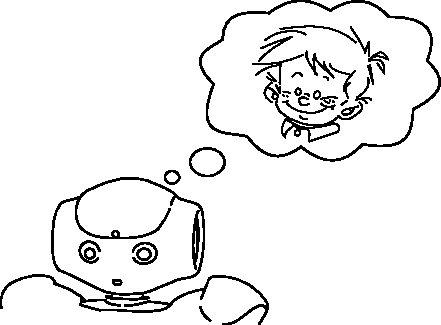
\includegraphics[width=0.8\columnwidth]{naoMM}
		\caption{Do I understand you ? }
	\end{minipage}
	\hfill
	\begin{minipage}[b]{.4\textwidth}
		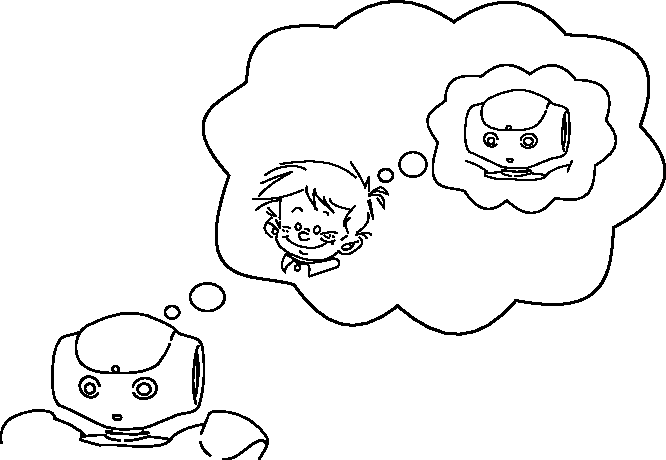
\includegraphics[width=0.8\columnwidth]{naoMM2}
		\caption{Do you understand me ? }
	\end{minipage}
	
\end{figure}
\end{frame}

\section*{The Activity}
\begin{frame}{The CoWriter interaction}
    \centering
    \textcolor{blue}{Learning by teaching} approach:
    \begin{tabular}{c c}
    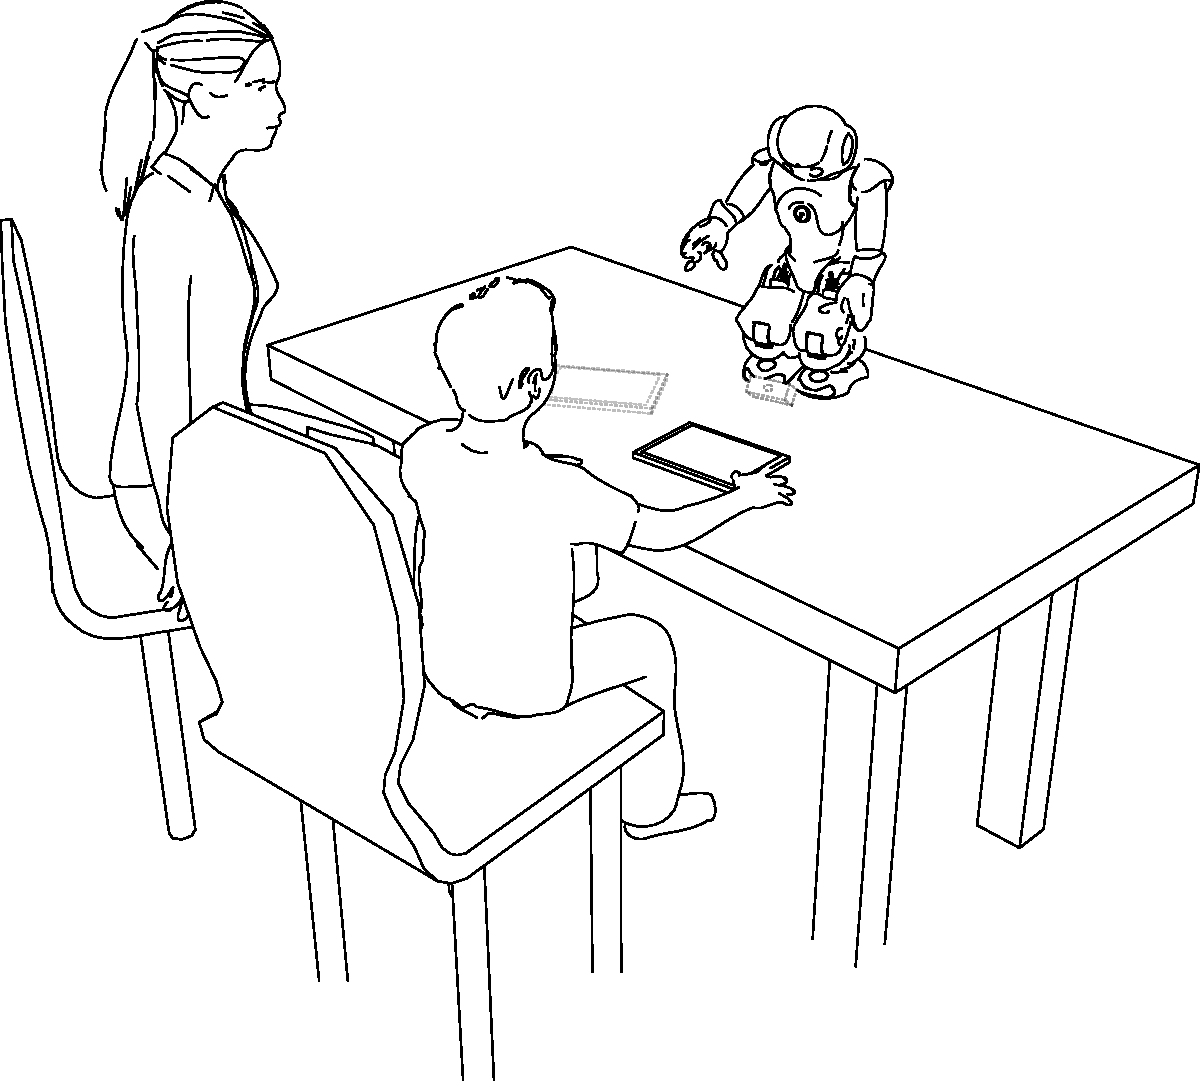
\includegraphics[width=0.5\columnwidth]{experimental_setup}
    &
    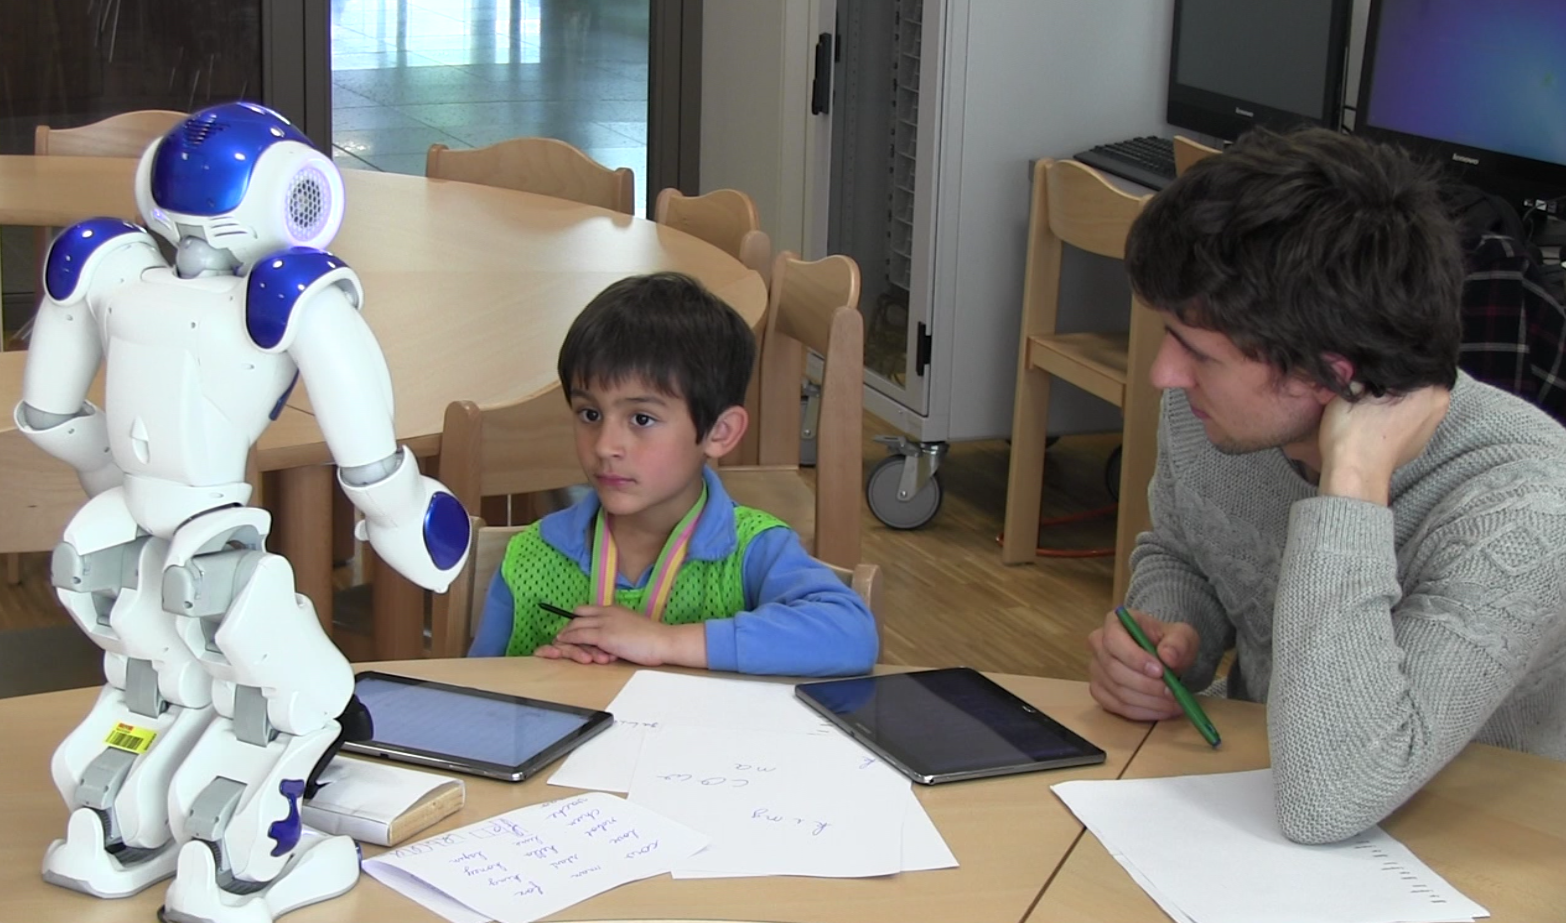
\includegraphics[width=0.45\columnwidth]{realSetup}
    \end{tabular}
    \begin{itemize}
    \item a \textcolor{blue}{physical robot} to induce a \textcolor{blue}{``prot\'eg\'e" effect}
    \item the robot is \textcolor{blue}{autonomous}
    \end{itemize}
\end{frame}

\begin{frame}{Observed issues}

{\bf The child needs to practice a lot to make progress}\\
{\bf Situations of misunderstanding}:
\begin{itemize}
\item When the child \textcolor{blue}{press unexpected button}
\item when the child is \textcolor{blue}{disengaged}
\item When the child \textcolor{blue}{does not perceive the difficulty (or progresses)} of the robot 
\item Incoherent \textcolor{blue}{visual behaviour} of the robot and the child 
\end{itemize}
\end{frame}

\begin{frame}

{\bf How to improve this interaction}:
\begin{itemize}
\item \textcolor{blue}{Long-term} interactions ?
\item \textcolor{blue}{Metric} to measure the progresses of the child ?
\item \textcolor{blue}{Perception of the progresses} of the robot ? % about how the child perceives...
\item \textcolor{blue}{Visual focus of attention} of the child ? 
\end{itemize}
\end{frame}

\begin{frame}{Study 1}

    \begin{itemize}
    \item {\bf Hypothesis}: We can do \textcolor{blue}{long-term interaction} with CoWriter
    \item {\bf Method}: \textcolor{blue}{Back-story}, 4 sessions of 1h, 1 session/week
    \item {\bf Measure}: \# of demo by session
    \item {\bf Result}: not decreasing
    \end{itemize}
    
    \begin{table}
    \centering
    \caption{\footnotesize Number of demonstrations provided by Vincent over the four sessions.}
    \begin{tabular}{lccccc}
        \toprule
        Session & S1 & S2 & S3 & S4 & Total\\ 
        Number of demonstrations & 23 & 34 & 52 & 46 & 155\\ 
        \bottomrule

    \end{tabular}
\end{table}

\tiny{Jacq, Lemaignan, Garcia, Dillenbourg \& Paiva, {\bf Building Successful Long-term Child-Robot Interactions in a Learning Context}, HRI 2016}\\
\tiny{Lemaignan, Jacq, Hood, Garcia, Paiva, \& Dillenbourg, {\bf Learning by Teaching a Robot: The Case of Handwriting}, RAM 2016}
    %\centering
    %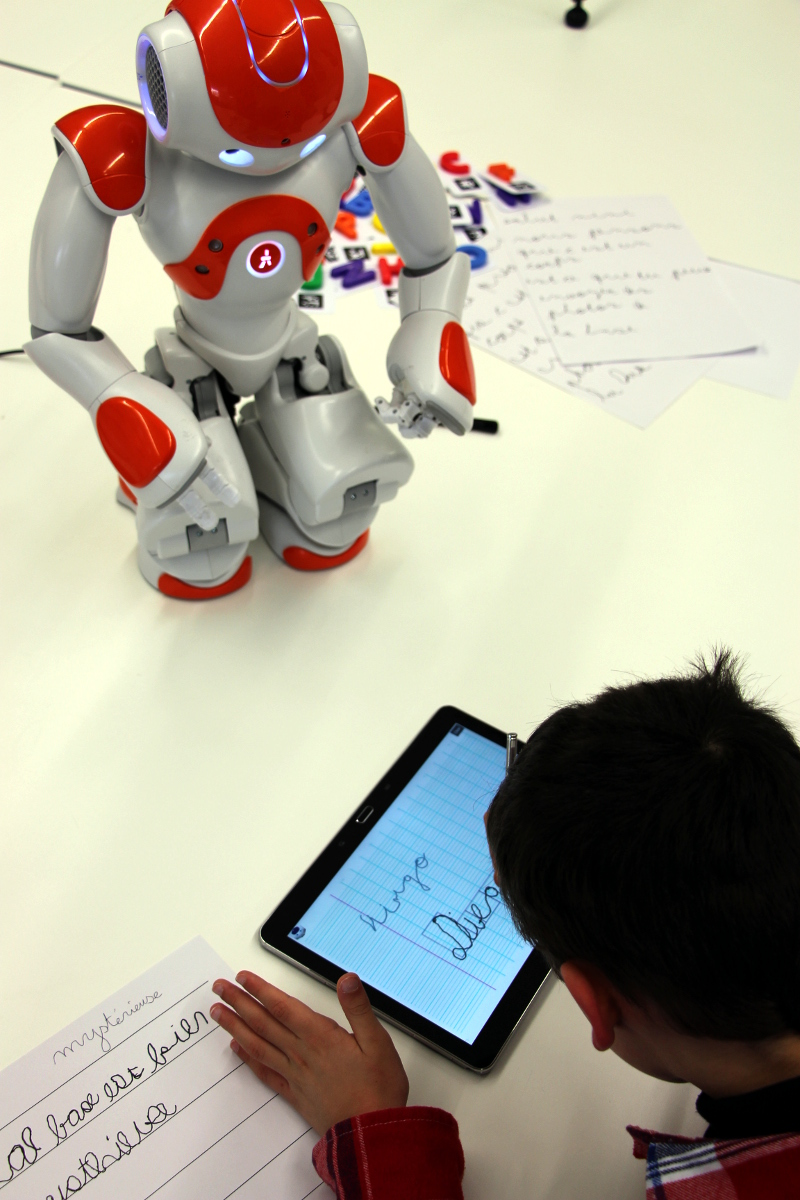
\includegraphics[width=0.15\columnwidth]{diego}
\end{frame}

%\begin{frame}
%	\centering    
%    Robot's handwriting
%    	\begin{tabular}{c c}
%    	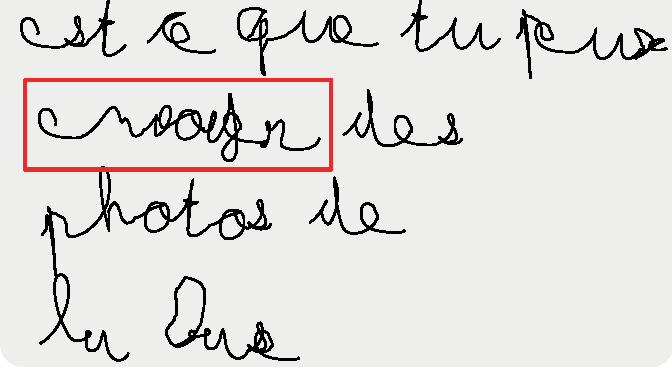
\includegraphics[width=0.45\columnwidth]{diego-initial-letter}
%    	&
%    	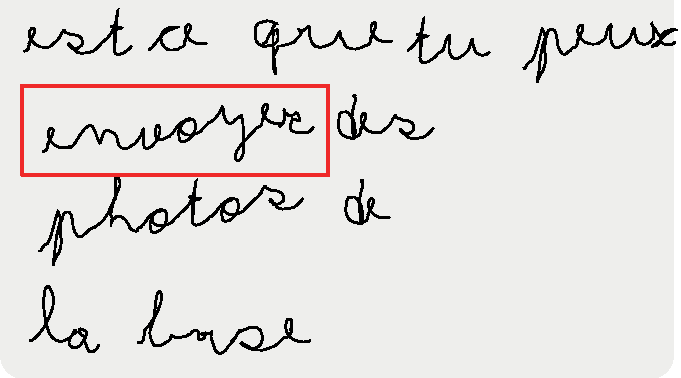
\includegraphics[width=0.45\columnwidth]{diego-final-letter}
%    	\\
%    	before Vincent's help & after Vincent's help
%    	\end{tabular}
%%\tiny{Jacq, Lemaignan, Garcia, Dillenbourg \& Paiva, {\bf Building Successful Long-term Child-Robot Interactions in a Learning Context}, HRI 2016}
%%\tiny{Lemaignan, Jacq, Hood, Garcia, Paiva, \& Dillenbourg, {\bf Learning by Teaching a Robot: The Case of Handwriting}, RAM 2016}
%\end{frame}

% we can observe the progress of the robot. but what about imporvement of the child ? can we measur them ?

\begin{frame}{Study 2}
    \begin{itemize}
    \item {\bf Hypothesis}: we can \textcolor{blue}{measure improvements}
    \item {\bf Method}: co-designed with therapist, no back-story, \\4 sessions of 45min, 1 session/week
    \item {\bf Measure}: \textcolor{blue}{distance between child's demo and ideal templates}
    \item {\bf Result}: we can \textcolor{blue}{separate legible and non-legible} letters
    \end{itemize}
    \begin{figure}
    	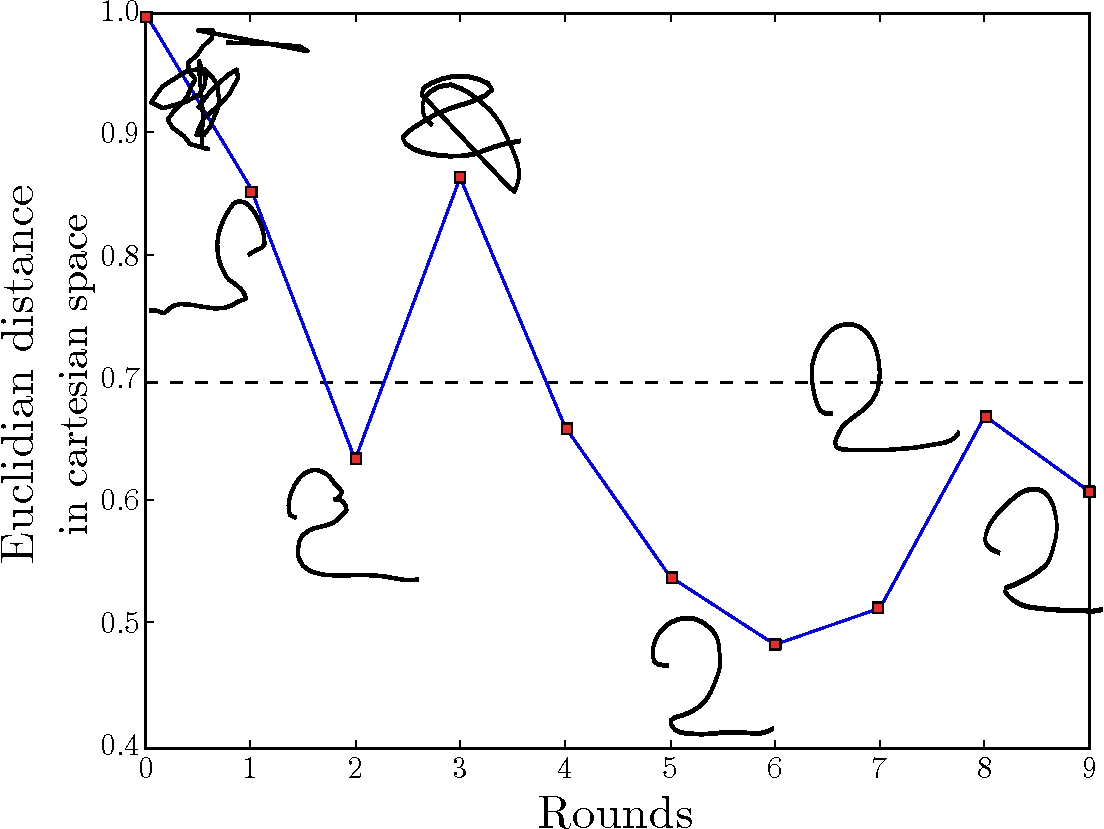
\includegraphics[width=0.4\columnwidth]{henry2}
    	\caption{Demonstrations of "2" provided by the child}
    \end{figure}
    %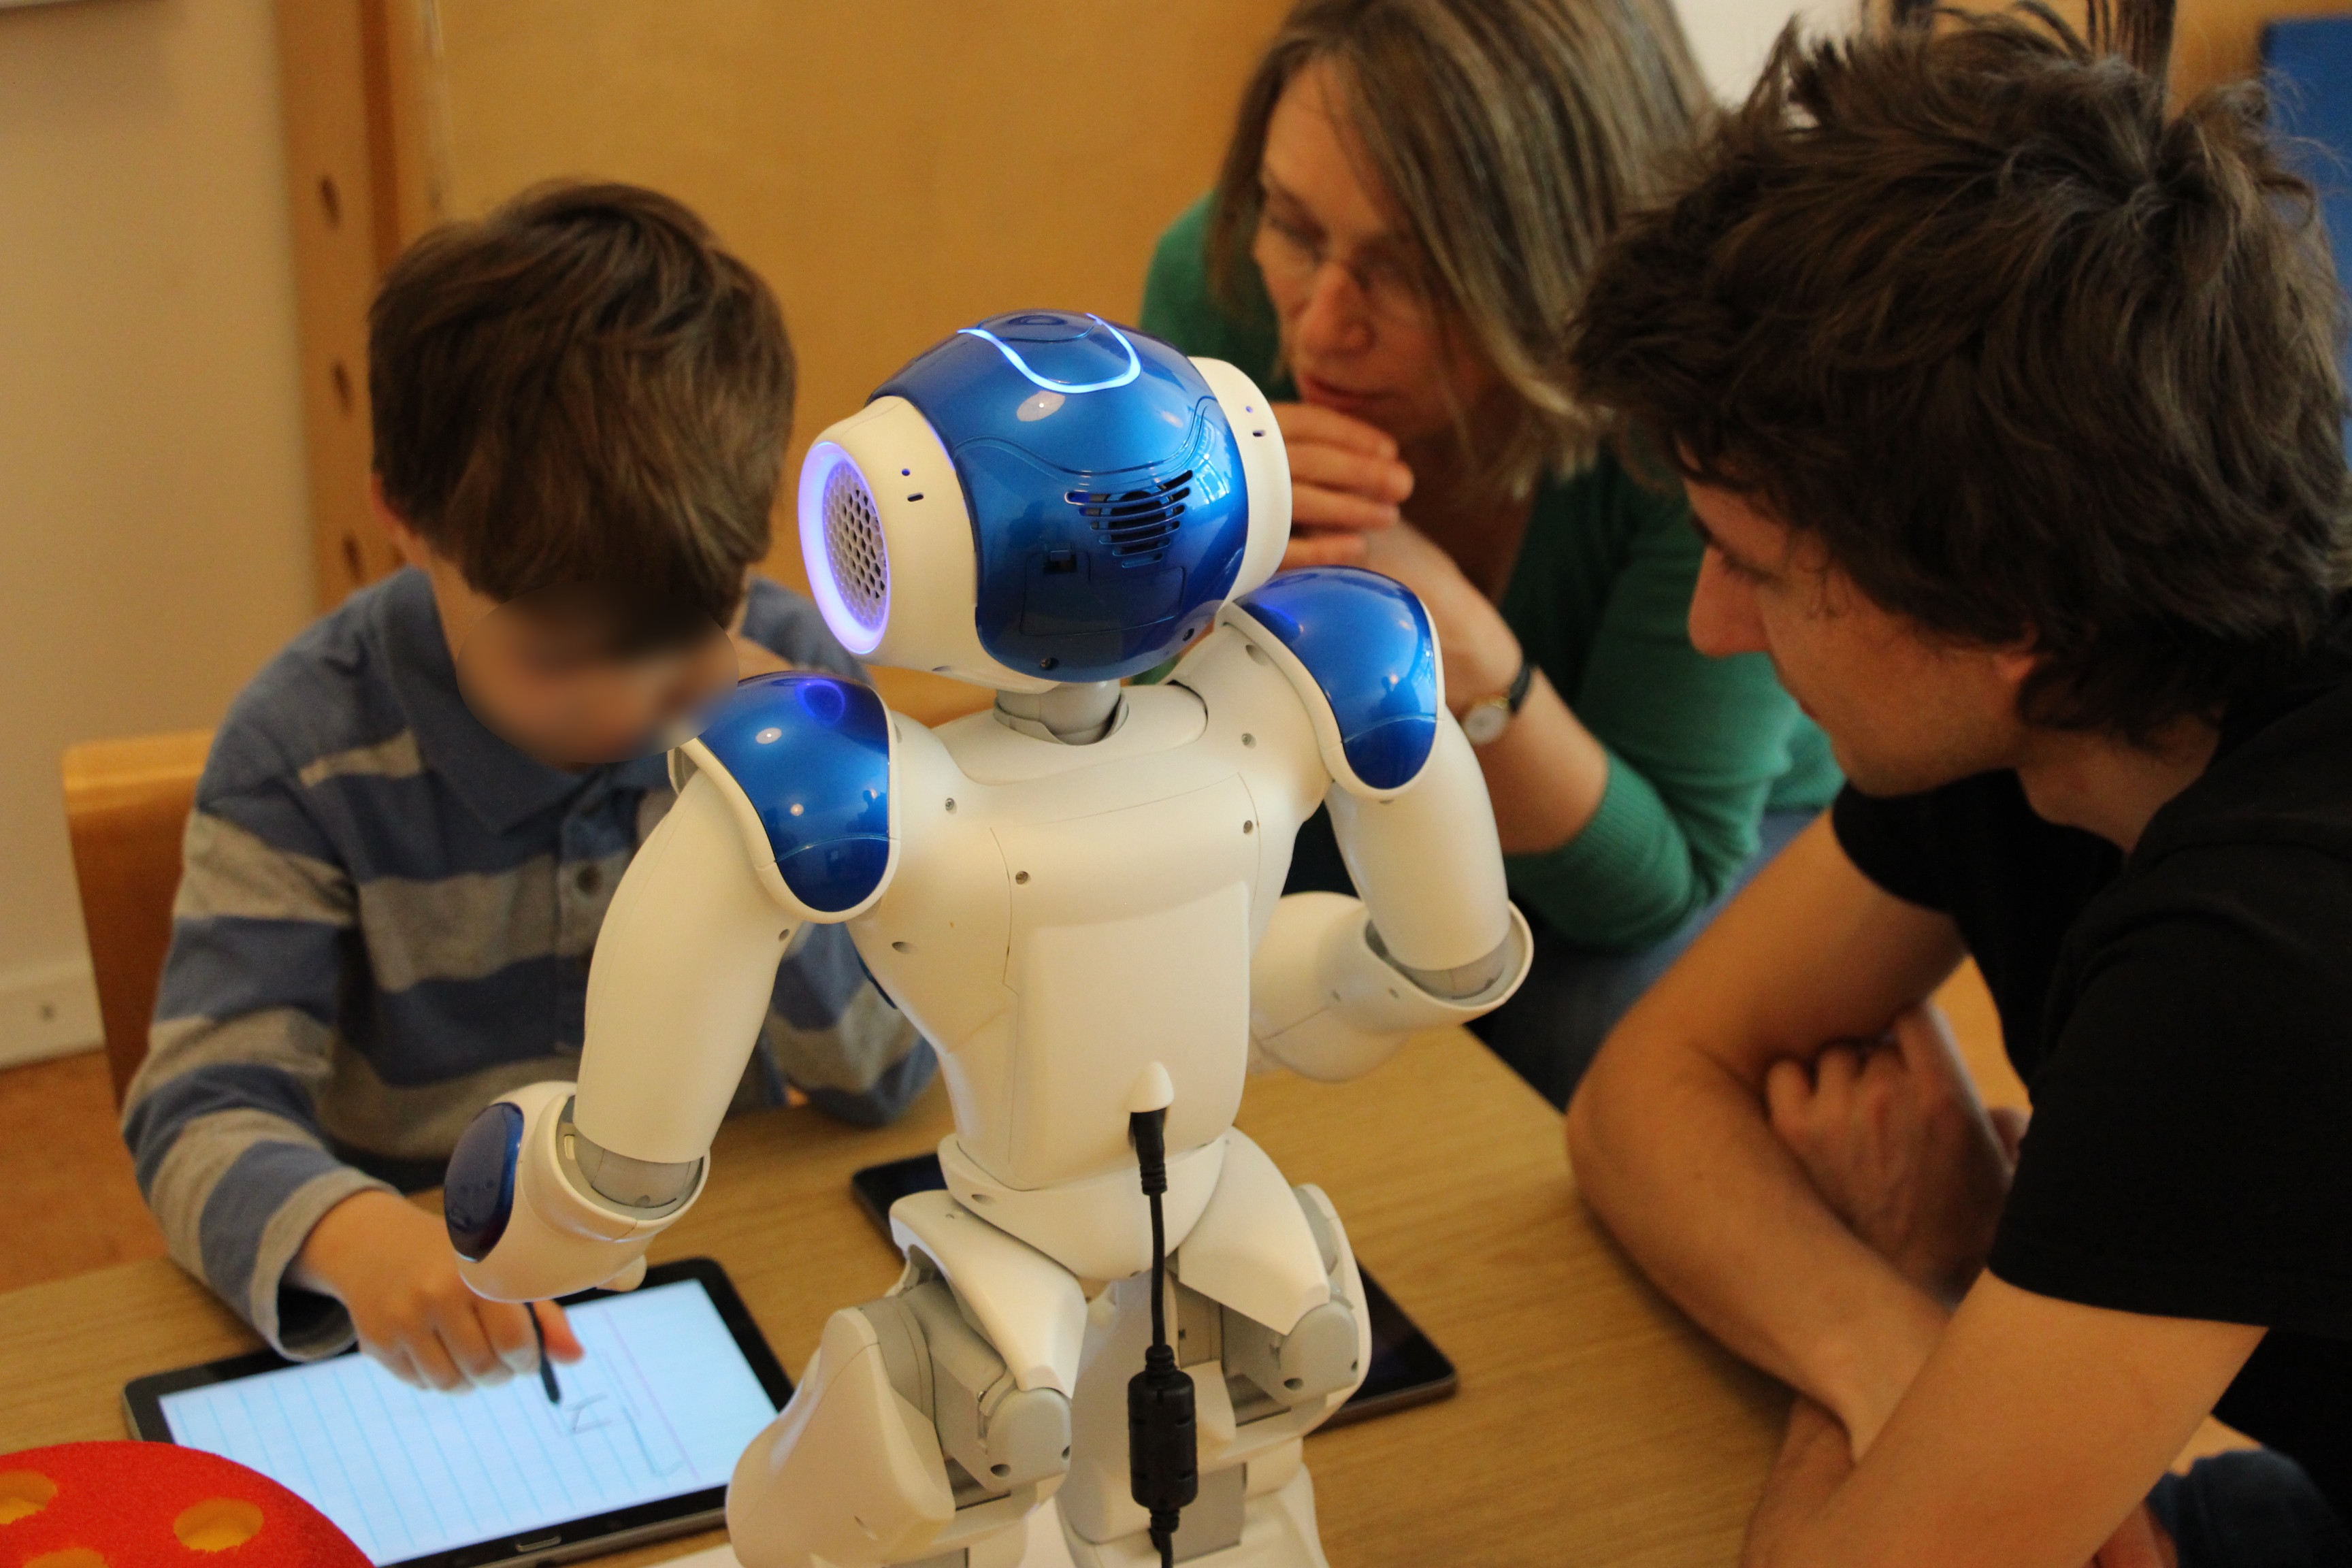
\includegraphics[width=0.25\columnwidth]{henry}
\tiny{Jacq, Lemaignan, Garcia, Dillenbourg \& Paiva, {\bf Building Successful Long-term Child-Robot Interactions in a Learning Context}, HRI 2016}\\
\tiny{Lemaignan, Jacq, Hood, Garcia, Paiva, \& Dillenbourg, {\bf Learning by Teaching a Robot: The Case of Handwriting}, RAM 2016}    

\end{frame}

% given this metric of the progress, is it possible to get information about the perception of the robot by the child as a begining learner without questionnary ?

\begin{frame}{Study 3}
    \begin{itemize}
    \item {\bf Hypothesis}: children \textcolor{blue}{perceive the progress of the robot}
    \item {\bf Method}: adding \textcolor{blue}{two buttons} for evaluation 
    \item {\bf Measure}: correlation between children evaluations and robot progress
    \item {\bf Result}: \textcolor{blue}{5 of 8 children} gave an evaluation \textcolor{blue}{correlated with robot's progress}
    \end{itemize}
    \centering
    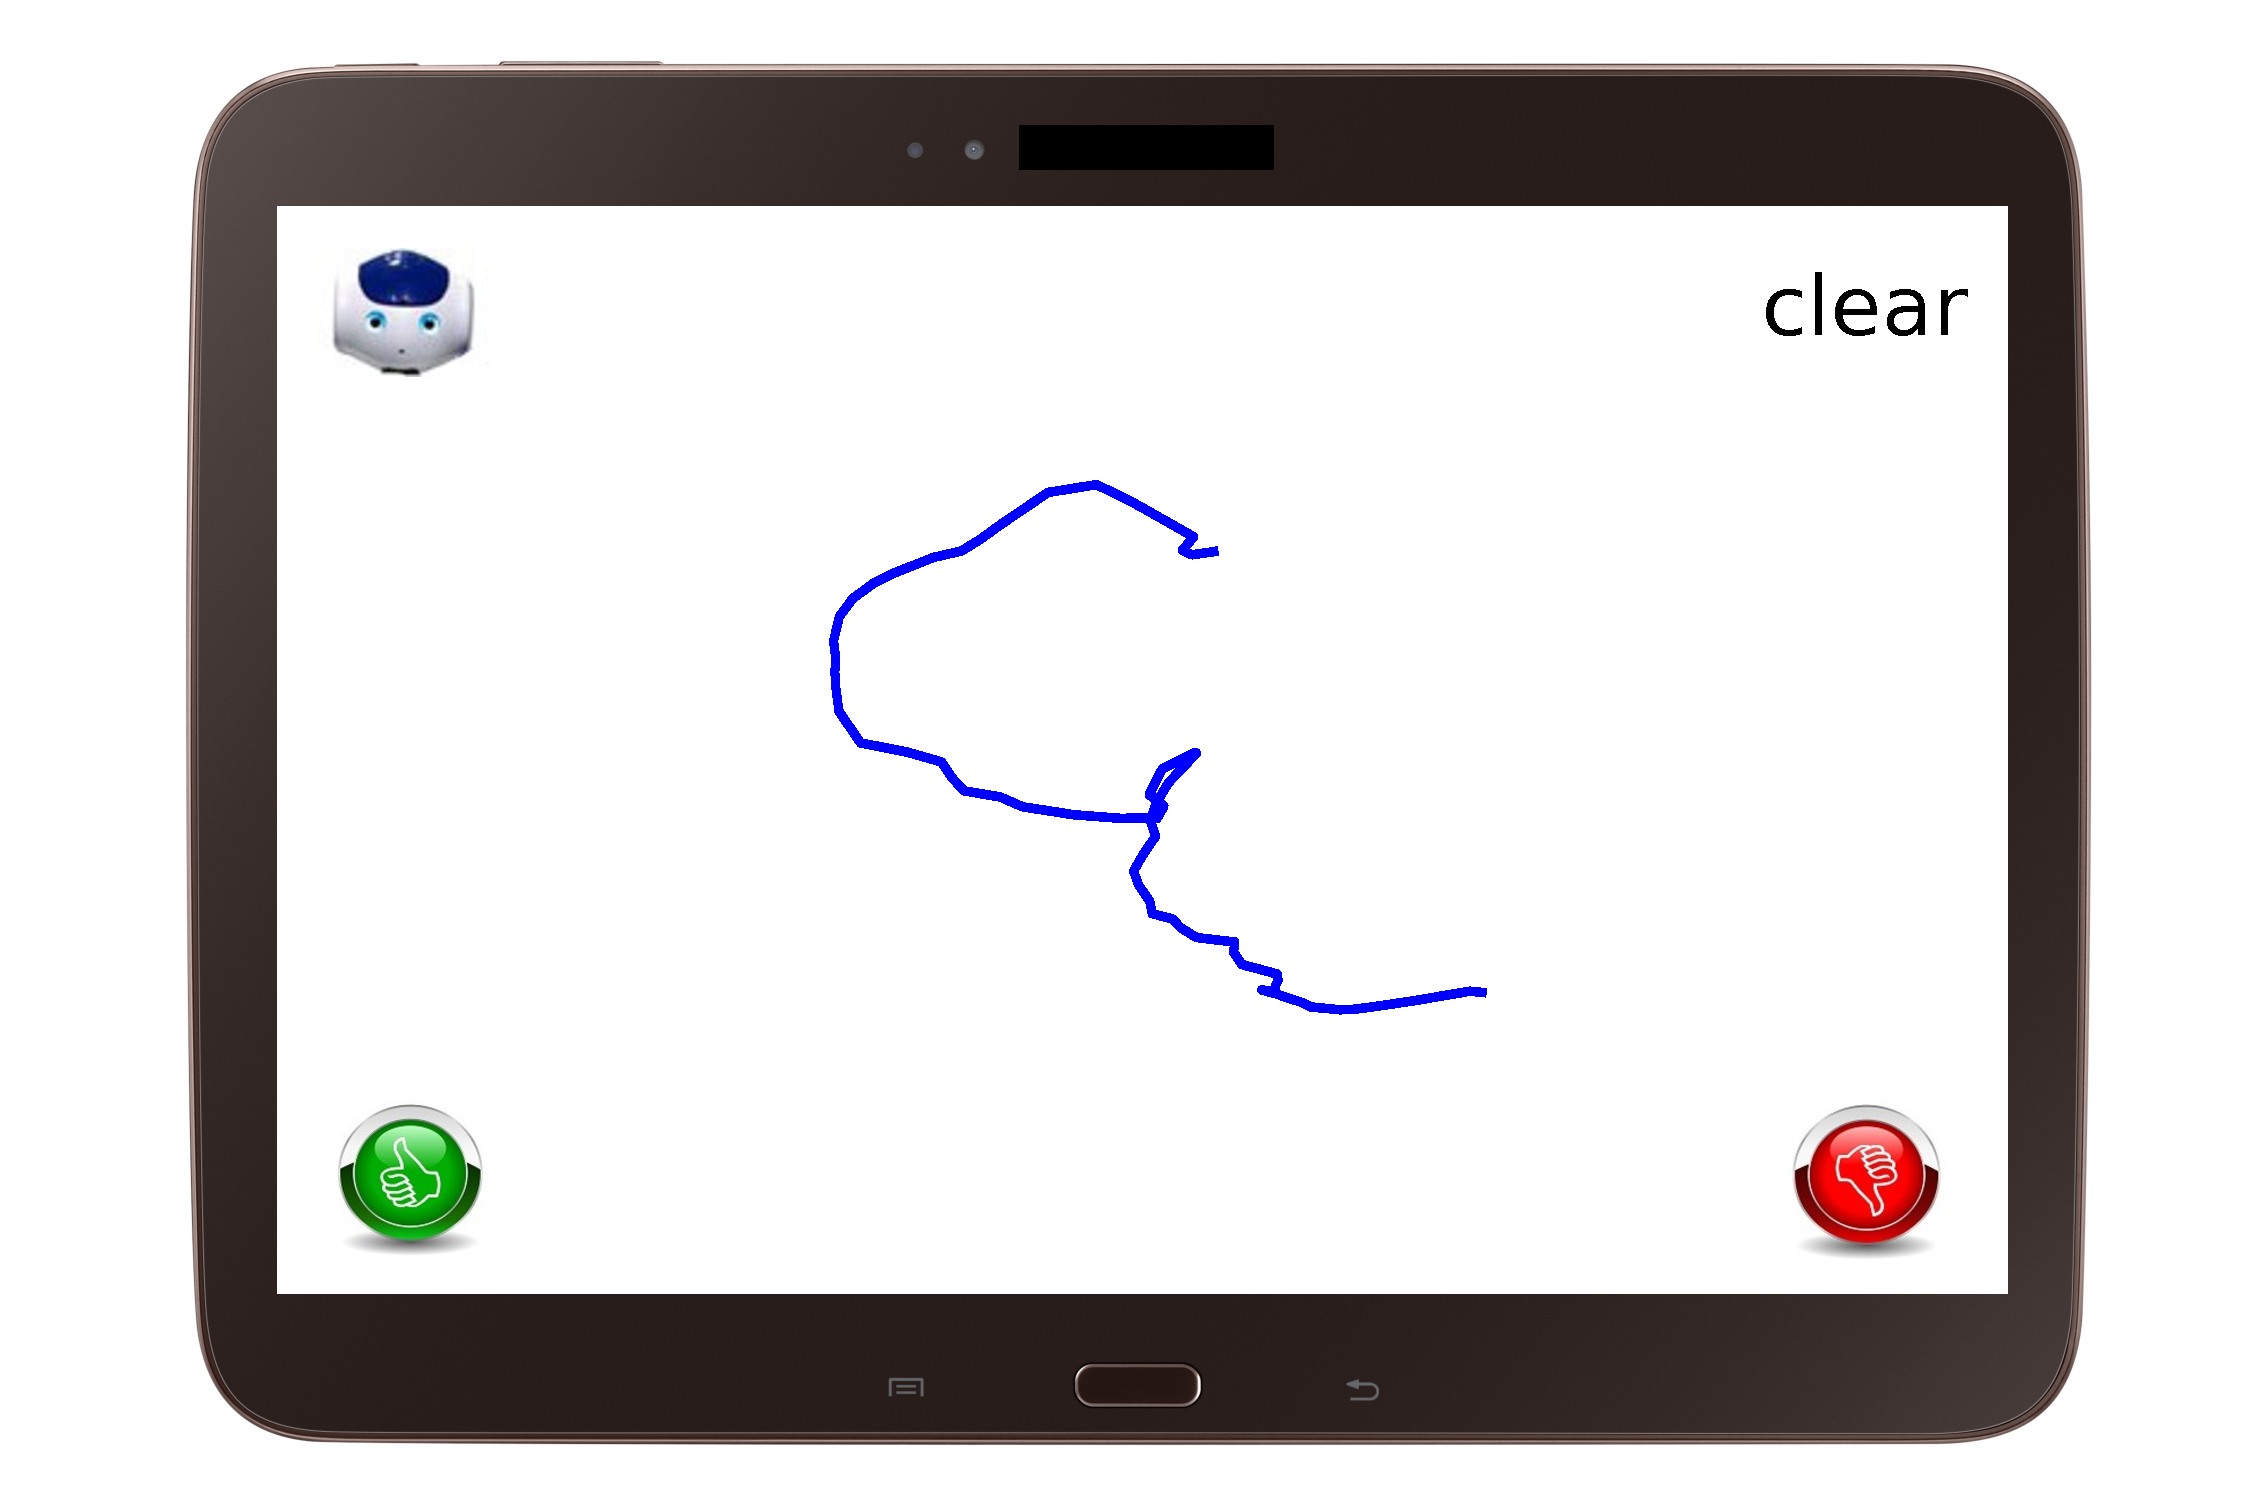
\includegraphics[width=0.35\columnwidth]{normandy_tablet}    

\begin{flushleft}
\tiny{Jacq, Lemaignan, Garcia, Dillenbourg \& Paiva, {\bf Building Successful Long-term Child-Robot Interactions in a Learning Context}, HRI 2016}\\
\tiny{Lemaignan, Jacq, Hood, Garcia, Paiva, \& Dillenbourg, {\bf Learning by Teaching a Robot: The Case of Handwriting}, RAM 2016}
\end{flushleft}
\end{frame}

\begin{frame}{Focus of attention}
    \begin{enumerate}
    \item \textcolor{blue}{Head-pose estimation}: Dlib's 68 facial features + 3D mesh of human face, RGB camera
    \item \textcolor{blue}{Visual focus of attention}: cone of 40\degree based on nose direction
    \item Object in focus = object in the cone
    \end{enumerate}
    \centering
    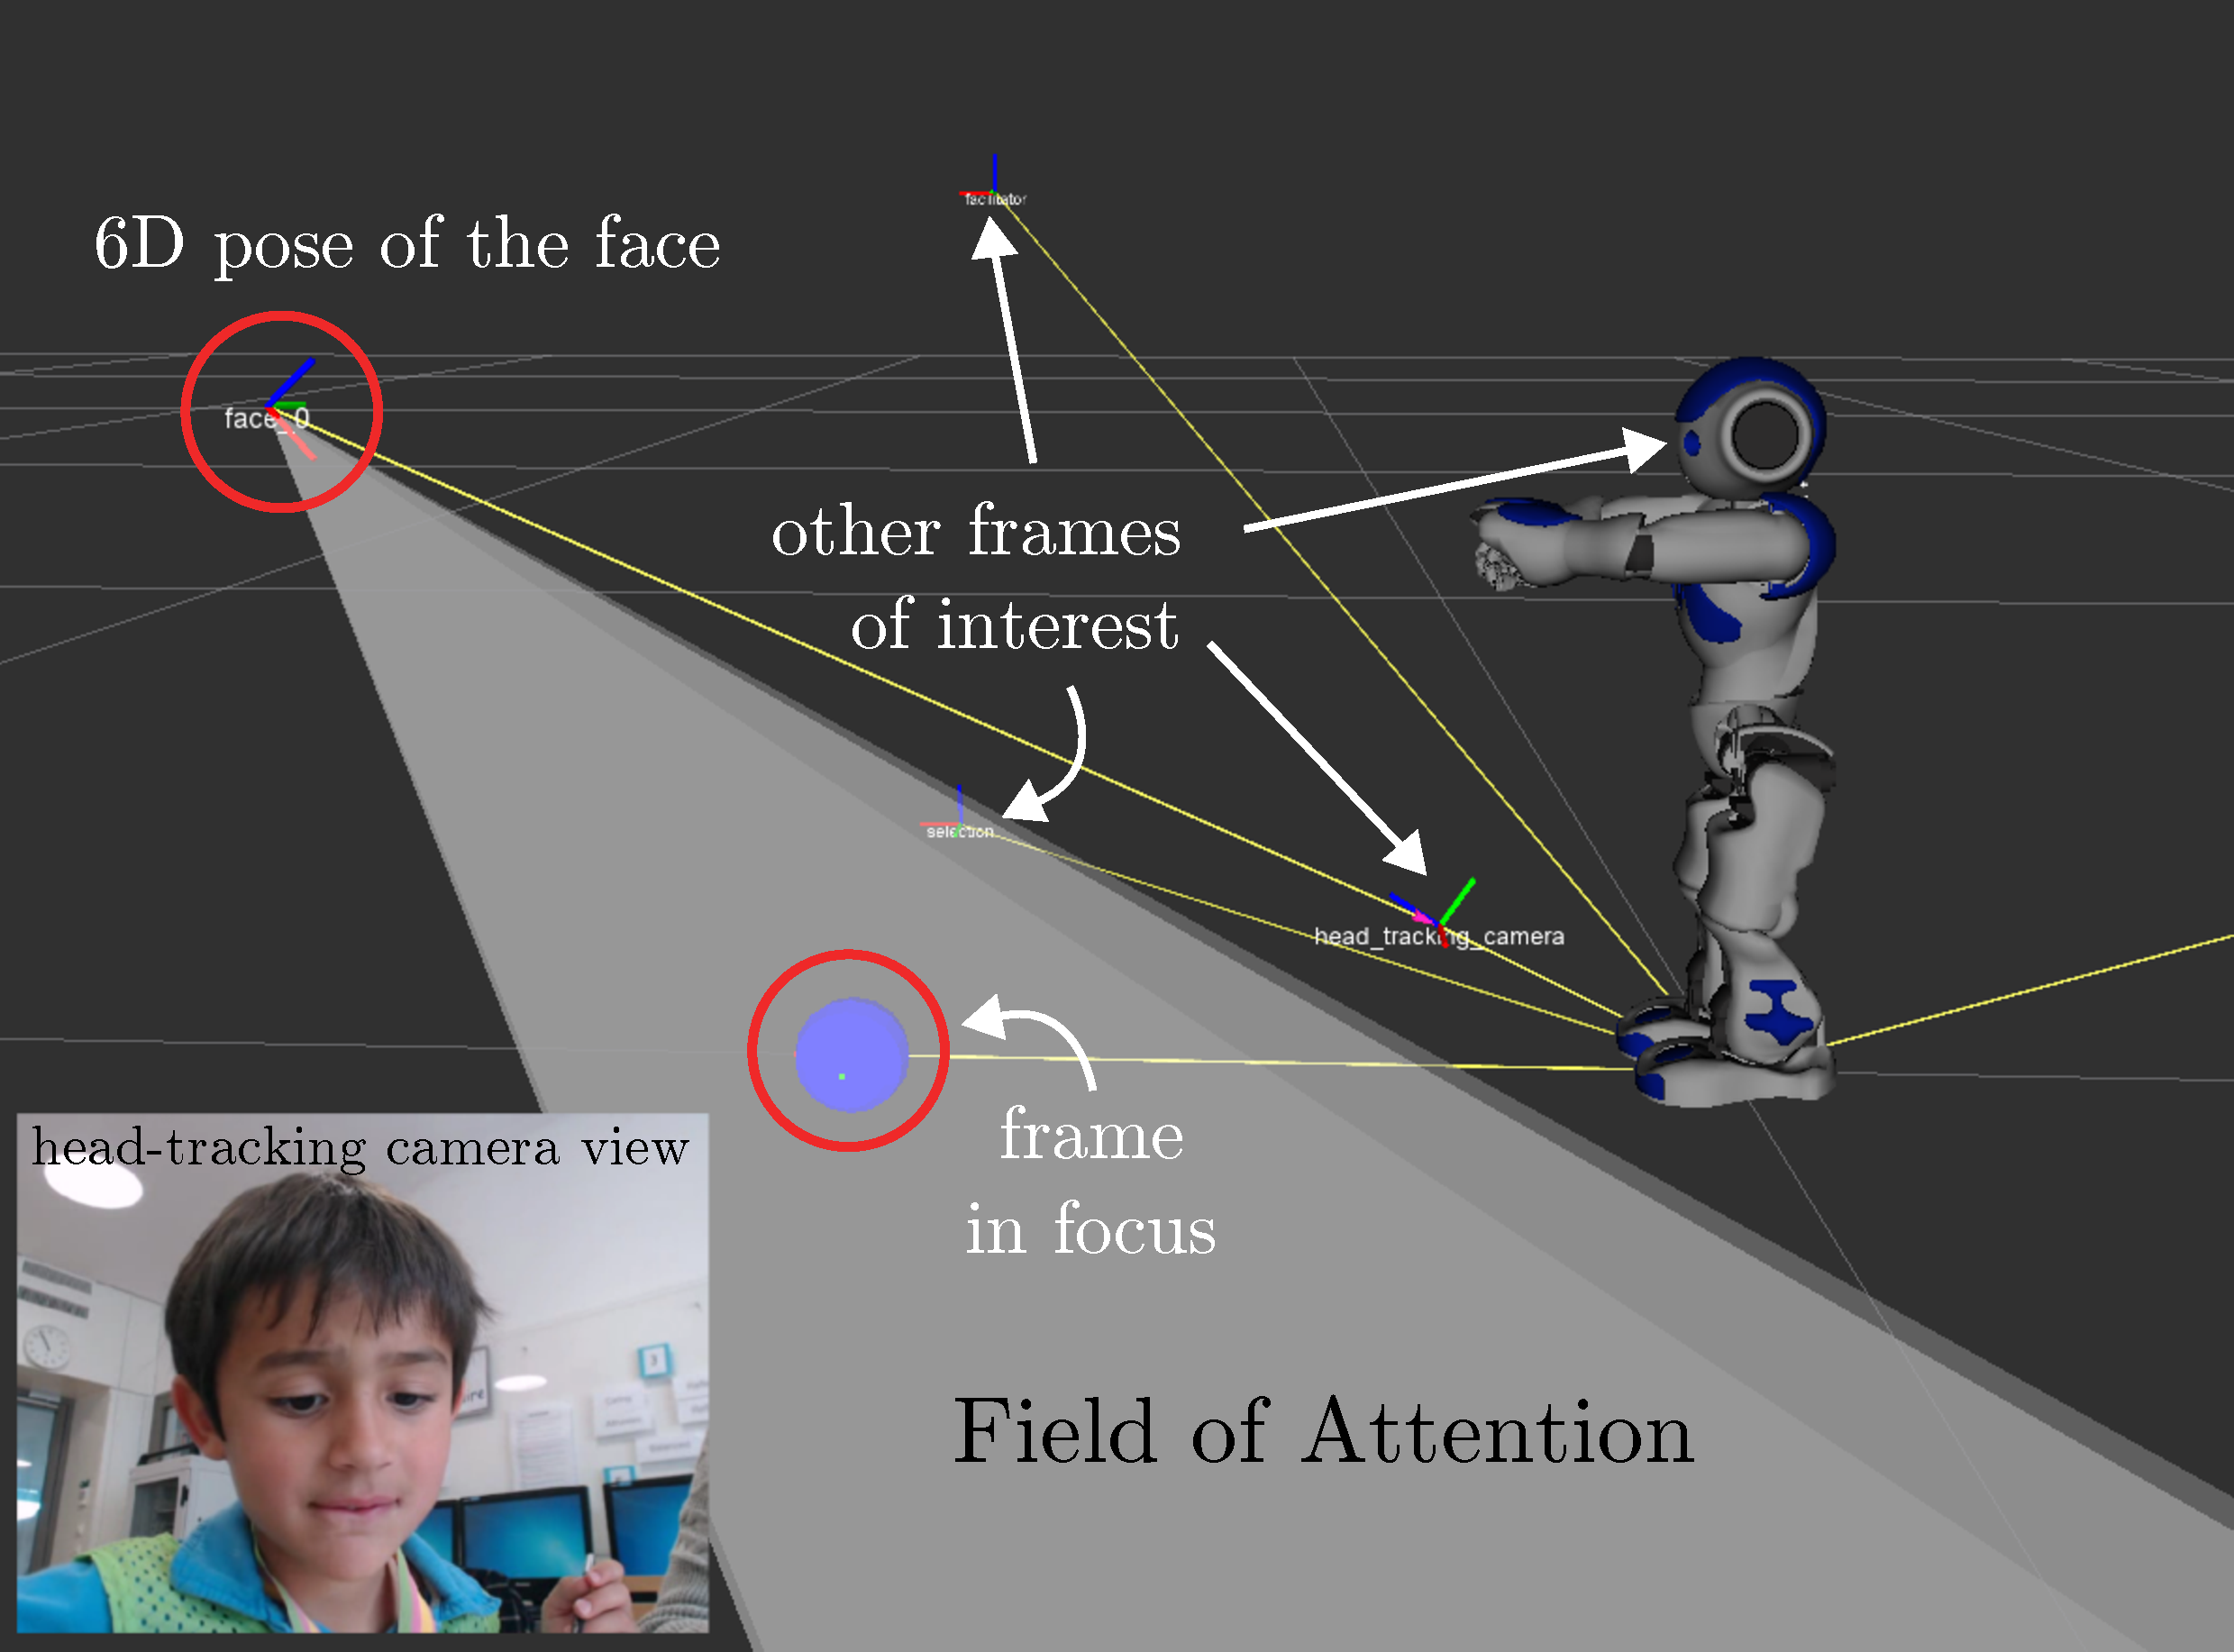
\includegraphics[width=0.4\columnwidth]{field_of_attention}
\end{frame}

\begin{frame}{Study 4}
    \begin{itemize}
    \item {\bf Hypothesis}: the \textcolor{blue}{estimation of the focus of attention} is \textcolor{blue}{robust enough} to be used for {\bf with-me-ness} estimation (with-me-ness = frequency the child has in focus objects he is expected to look at).
    \item {\bf Method}: 6 subjects filmed during activity
    \item {\bf Measure}: correlation between \textcolor{blue}{human annotation and estimation} of the system
    \item {\bf Result}: \textcolor{blue}{r=0.46}, good estimator of humans perception\\
    \end{itemize}
    
\tiny{Lemaignan, Garcia, Jacq, Dillenbourg {\bf From Real-time Attention Assessment to “With-me-ness” in Human-Robot Interaction}, HRI 2016}
\end{frame}

\begin{frame}

{\bf to summarize}:
\begin{itemize}
\item (S1) \textcolor{blue}{Long-term} interactions
\item (S2) \textcolor{blue}{Metric} to measure the progresses of the child
\item (S3) Information about the \textcolor{blue}{perception of the progresses} of the robot % about how the child perceives...
\item (S4) Estimation of the \textcolor{blue}{visual focus of attention} in real time
\end{itemize}
\end{frame}

\begin{frame}{Project for incoming years}
My goal is to develop a \textcolor{blue}{cognitive architecture} that 
\begin{itemize}
\item \textcolor{blue}{takes as input} progress of the child, focus of attention, perception of robot's progress...
\item builds \textcolor{blue}{models of agents} (robot, child, robot perceived by child) 
\item \textcolor{blue}{detects and repairs misunderstanding}
\end{itemize}
\end{frame}

%%%%%%%%%%%%%%%%%%%%%%%%%%%%%%%%%%%%%%%%%%%%%%%%%%%%%%%%%%%%%%%%%%%%%%%%%%%%%%%

\section*{Mutual modelling}


\begin{frame}{Mutual modelling}
\begin{figure}[!tbp]
	\begin{minipage}[b]{.4\textwidth}
		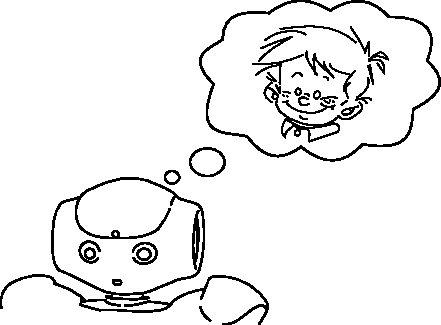
\includegraphics[width=0.8\columnwidth]{naoMM}
		\caption{\textcolor{blue}{$M_R\left[\textit{C}\right]$} (1st level) }
	\end{minipage}
	\hfill
	\begin{minipage}[b]{.4\textwidth}
		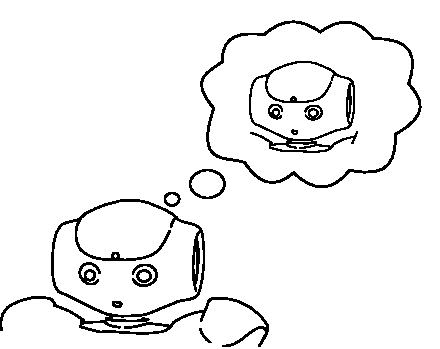
\includegraphics[width=0.8\columnwidth]{naoMM4}
		\caption{\textcolor{blue}{$M_R\left[\textit{R}\right]$} (1st level)}
	\end{minipage}
	%\hfill
	%\begin{minipage}[b]{.4\textwidth}
	%	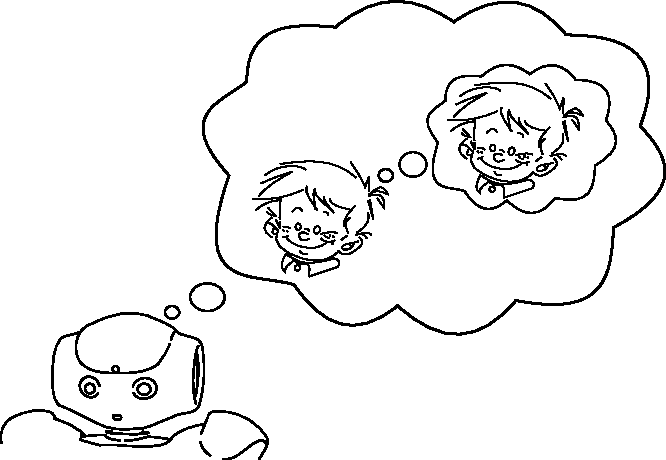
\includegraphics[width=0.8\columnwidth]{naoMM3}
	%	\caption{\textcolor{blue}{$M_R\left[\textit{C,C}\right]$} (2nd level)}
	%\end{minipage}
	\hfill
	\begin{minipage}[b]{.4\textwidth}
		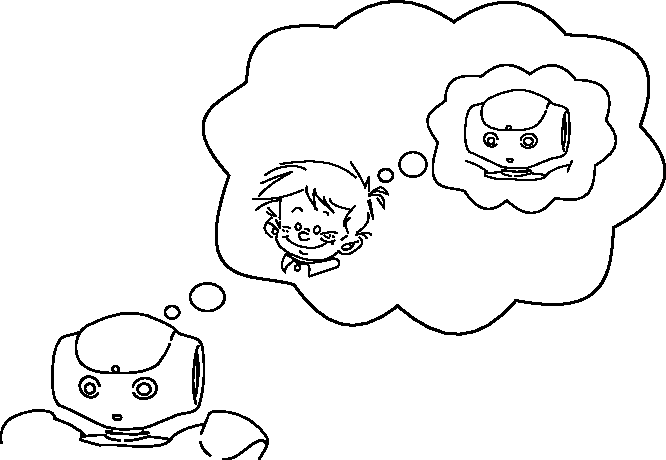
\includegraphics[width=0.8\columnwidth]{naoMM2}
		\caption{\textcolor{blue}{$M_R\left[\textit{C,R}\right]$} (2nd level)}
	\end{minipage}
	
\end{figure}
\end{frame}

\begin{frame}{Using models}
\centering
\begin{figure}
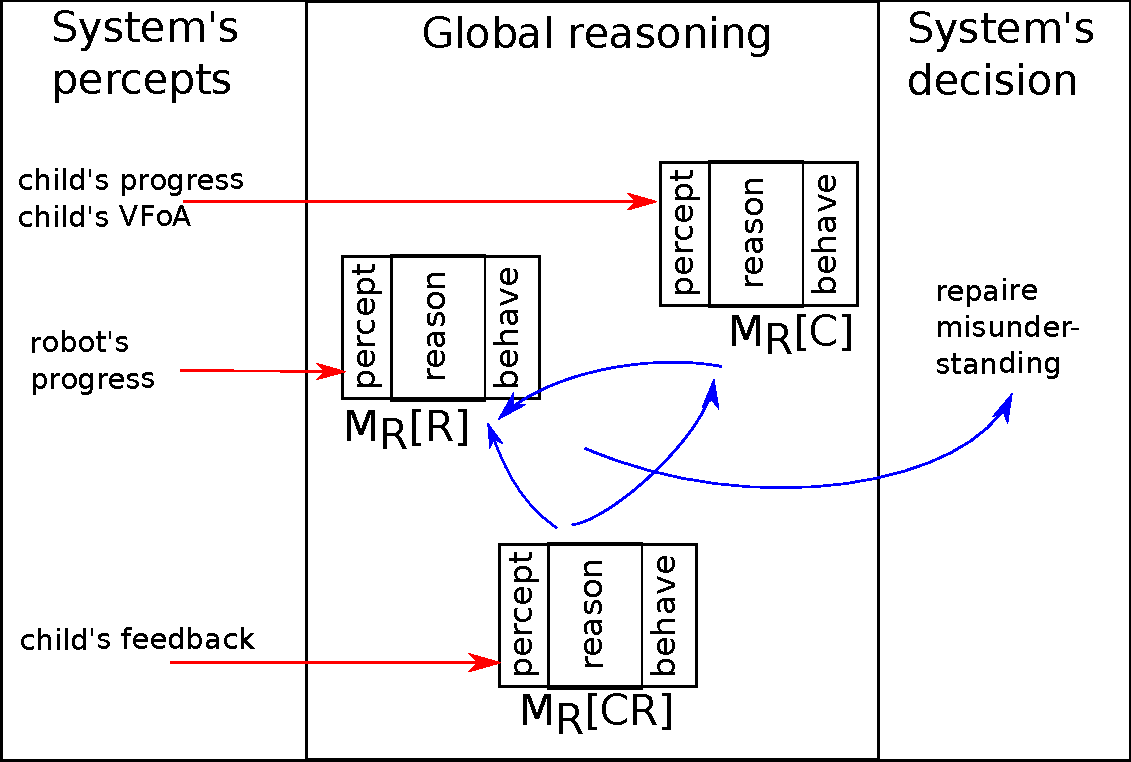
\includegraphics[width=0.8\columnwidth]{archi_general}
\end{figure}
\end{frame}

\begin{frame}{Misunderstanding (by the robot)}
When the robot misunderstands the human:
\centering
\begin{figure}
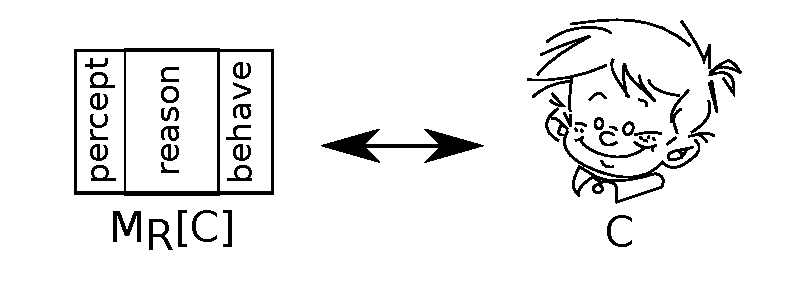
\includegraphics[width=0.8\columnwidth]{true_mis11}
\end{figure}

Prediction error:
\huge
\textcolor{blue}{$$\Delta \left(P^{t+1}_R\left[\textit{C}\right] ; M^{t+1}_R\left[\textit{C}\right]\right)$$}
\end{frame}

\begin{frame}{Misunderstanding (by the robot)}
When the robot misunderstands how the human perceives it:
\centering
\begin{figure}
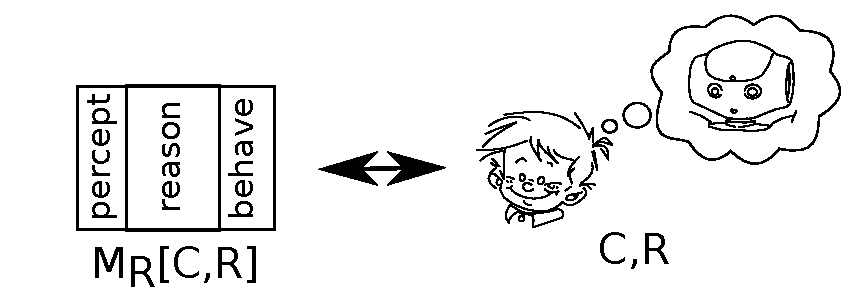
\includegraphics[width=0.8\columnwidth]{true_mis12}
\end{figure}
Prediction error:
\huge
\textcolor{blue}{$$\Delta \left(P^{t+1}_R\left[\textit{C,R}\right] ; M^{t+1}_R\left[\textit{C,R}\right] \right)$$}
\end{frame}

\begin{frame}{Misunderstanding (by the child)}
When the human misunderstands the robot:
\centering
\begin{figure}
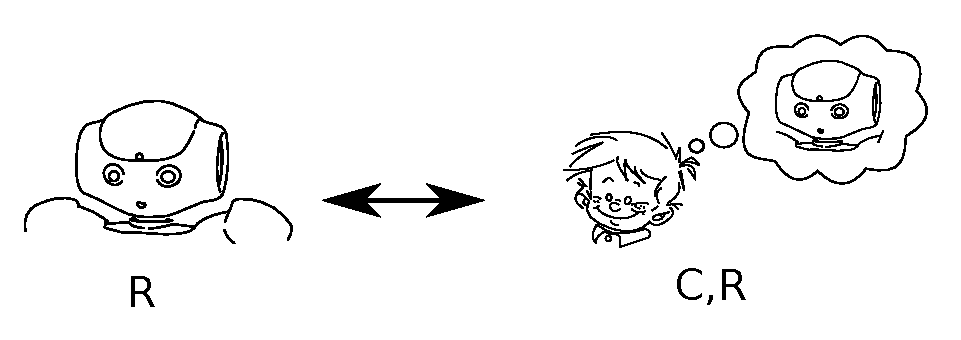
\includegraphics[width=0.9\columnwidth]{true_mis2}
\end{figure}

Child's perception error:
\huge
\textcolor{blue}{$$\Delta \left( M^t_R\left[\textit{R}\right] ; M^t_R\left[\textit{C,R}\right]\right)$$}
\end{frame}

%%%%%%%%%%%%%%%%%%%%%%%%%%%%%%%%%%%%%%%%%%%%%%%%%%%%%%%%%%%%%%%%%%%%%%%%%%%%%%%

\section*{Cognitive architecture}

\begin{frame}{Cognitive architecture}
\centering
\begin{figure}
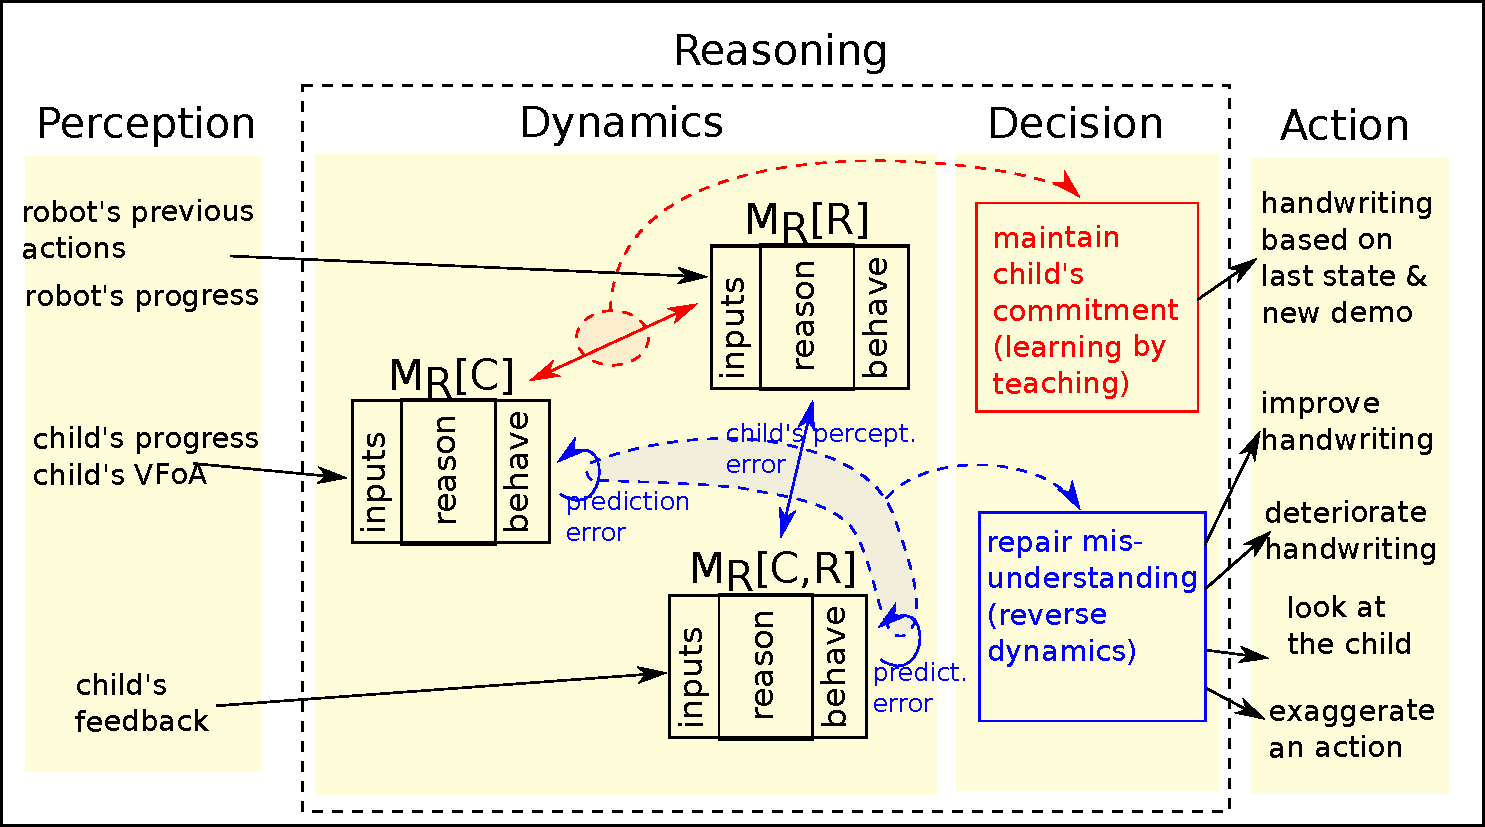
\includegraphics[width=1.\columnwidth]{final_archi}
\end{figure}
\end{frame}


%%%%%%%%%%%%%%%%%%%%%%%%%%%%%%%%%%%%%%%%%%%%%%%%%%%%%%%%%%%%%%%%%%%%%%%%%%%%%%%

\section*{Experimental studies}

\begin{frame}{Parametrization}

{\bf How to train the robot}:
\begin{itemize}
\item \textcolor{blue}{learning the dynamic} between variables of different models
\item learning how to \textcolor{blue}{make decisions}
\end{itemize}
\end{frame}

\begin{frame}{Parametrization}

{\bf Decision making}
\begin{enumerate}
\item {\bf Wizard-of-Oz}: A human makes decisions; the robot learns. %The wizard only has access to what the robot uses to make decision, namely the 3 models $M_C\left[CR\right]$, $M_C\left[C\right]$ and $M_C\left[R\right]$ containing the current values of variables. In order to explicitly link decision of the wizard to the cause of his decision, an idea would be to use a graphical interface where he could select the causes (for example a child's perception error) and then select an action (for example an exaggeration of the previous action).
\item {\bf Mixed-initiative}: The robot makes suggestions; a human agrees or disagrees
\item {\bf Autonomous}: The robot makes decisions
\end{enumerate}
\end{frame}

\begin{frame}{Verification}

\only<1>{
{\bf Hypothesis}:
\begin{itemize}
\item \textit{Decisions made with a second level of modelling aiming to maintain mutual understanding, \textcolor{blue}{improve the quality of human-robot interactions}.}
\end{itemize}
{\bf This can be developed in two sub-hypothesis}
}
\only<2>{
{\bf Sub-hypothesis 1}:
\begin{itemize}
\item \textit{The second level of modelling enable \textcolor{blue}{different decisions} from a robot that does not have this second level}.
\end{itemize}
{\bf Experimental approach}:
\begin{itemize}
\item \textcolor{blue}{Human judge} and/or \textcolor{blue}{Objective comparison}. Short experiments, Large number of subjects. Control: 1st level MM
\end{itemize}
}
\only<3>{
{\bf Sub-hypothesis 2}:
\begin{itemize}
\item \textit{The quality of human-robot interactions is \textcolor{blue}{greater} with the robot that has the second level of modelling}.
\end{itemize}
{\bf Experimental approach}:
\begin{itemize}
\item \textcolor{blue}{Long-term experiments} in real educational/therapeutic context. Small number of subjects. Control: no MM, 1st level MM 
\end{itemize}
}
\end{frame}

%%%%%%%%%%%%%%%%%%%%%%%%%%%%%%%%%%%%%%%%%%%%%%%%%%%%%%%%%%%%%%%%%%%%%%%%%%%%%%%

\section*{Conclusion}

\begin{frame}{Conclusion}

\only<1>{
{\bf I have}:
\begin{itemize}
\item a rich educational interaction where we can extract relevant information about child's mind
\end{itemize}}

\only<2>{

{\bf I have}:
\begin{itemize}
\item a rich educational interaction where we can extract relevant information about child's mind
\end{itemize}

{\bf I want to develop and evaluate an architecture}:
\begin{itemize}
\item that uses this information in order to detect and repair misunderstandings
\end{itemize}}

\only<3>{
{\bf I have}:
\begin{itemize}
\item a rich educational interaction where we can extract relevant information about child's mind
\end{itemize}

{\bf I want to develop and evaluate an architecture}:
\begin{itemize}
\item that uses this information in order to detect and repair misunderstandings
\end{itemize}

{\bf I believe}:
\begin{itemize}
\item such an architecture could be easily generalised to other human-robot interaction
\end{itemize}}

\end{frame}

\begin{frame}{Thank you !}
	\begin{figure}
        \centering
        \includegraphics[width=1.\columnwidth]{questions}
    \end{figure}
\end{frame}


\begin{frame}{Decision making}
\begin{table}
\centering
\small
\renewcommand{\arraystretch}{0.9}
\begin{tabular}{|l|l|}
\hline
$M^{t}_R\left[\textit{C}\right]$ & provides robot with positive feedback\\
\hline
$M^{t+1}_R\left[\textit{R}\right]$ & current level of handwriting = 0.1\\
\hline
$M^{t+1}_R\left[\textit{C,R}\right]$ & current level of handwriting = 0.7\\
\hline
$\Delta=0.6 \geq \Theta$ & high error, must be repaired\\
\hline
Reverse dynamic & \textit{what leads to small level of handwriting in} $M^{t}_R\left[\textit{C,R}\right]$ ?\\
\hline
$M^{t+1}_R\left[\textit{C,R}\right]$ & current level of handwriting = 0.1\\
\hline
$P^{t}_R\left[\textit{C}\right]$ & child give negative feedback\\
\hline
$P^{t-1}_R\left[\textit{R}\right]$ & robot writes letters with very poor style\\
\hline
$P^{t-1}_R\left[\textit{C}\right]$ & child is looking at the tablet\\
\hline
$P^{t-2}_R\left[\textit{R}\right]$ & robot is looking at the tablet\\
\hline
$P^{t-2}_R\left[\textit{C}\right]$ & child is looking at the robot\\
\hline
$P^{t-3}_R\left[\textit{R}\right]$ & robot is looking at the child\\
\hline
Decision 1 & robot looks at the child\\
\hline
$M^{t+2}_R\left[\textit{C}\right]$ & child is looking at the robot\\
\hline
Decision 2 & robot looks at the tablet\\
\hline
$P^{t+3}_R\left[\textit{C}\right]$ & child is looking at the tablet\\
\hline
Decision 3 & robot writes letters with very poor style\\
\hline
\end{tabular}
\caption{How to make decision in order to repair child's perception error}
\label{child_err_2}
\end{table}
\end{frame}

\begin{frame}{Encoding dynamic of an agent}
\begin{itemize}
\item a node encodes the value (truth or intensity) of a variable between 0 and 1
\item when the change of the value of one node is followed by the change of value of another one, we create/reinforce a link between these nodes. (\sim Hebbian learning)
\end{itemize}
\end{frame}

\begin{frame}{Quality of interaction}
\begin{itemize}
\item With-me-ness
\item $\sharp$ of demonstrations over longer term (>> 4 session)
\item Duration of ``free" session
\item Human judge (video annotation)
\item Progress of the child
\end{itemize}
\end{frame}

\end{document}






